\documentclass[10pt,aspectratio=169]{beamer}

% All the boilerplate is in ccaslides.sty
% Note that this also pulls in a custom vogtwidebar.sty
\usepackage{ccaslides}

\author{Ji\v{r}\'i Lebl}

\institute[OSU]{%
Departemento pri Matematiko de Oklahoma {\^S}tata Universitato}

\title{Cultivating Complex Analysis:\\%
Harmonic functions\\%
Dirichlet problem in a disc and the Poisson kernel (7.2.1)}

\date{}

\begin{document}

\begin{frame}
\titlepage
\end{frame}

\begin{frame}
\textbf{Dirichlet problem:}
\pause
\medskip

$U \subset \C$ open,
\pause
\quad
$u \colon \partial U \to \R$ continuous,
\quad
\pause
find a continuous $f \colon \widebar{U} \to \R$
harmonic on $U$, such that $f|_{\partial U} = u$.

\medskip
\pause

Solvable for many $U$, but not all.
\pause
But solution unique if it exists:
\pause

\begin{proposition}
Suppose $U \subset \C$ is a bounded domain, $f,g \colon \widebar{U} \to \R$
are continuous functions harmonic on $U$,
such that $f = g$ on $\partial U$.
Then $f=g$ on $U$.
\end{proposition}

\pause
\textbf{Proof:} Maximum principle (second version) on $f-g$. \qed

\medskip
\pause

On an unbounded domain, solution need not be unique.

\medskip

\textbf{Exercise:} The Dirichlet problem does not have a unique solution on
the upper half plane $\bH$.
\end{frame}

\begin{frame}
The Poisson kernel
for the unit disc $\D \subset \C$ is
\begin{equation*}
P_r(\theta)
= \frac{1}{2\pi} \frac{1-r^2}{1+r^2-2r \cos \theta}
= \frac{1}{2\pi}
\Re \left( \frac{1+re^{i\theta}}{1-re^{i\theta}}\right) ,
\qquad \text{for $0 \leq r < 1$.}
\end{equation*}

As a function of $z=re^{i\theta}$:
\begin{equation*}
\frac{1}{2\pi} \Re \left( \frac{1+z}{1-z}\right)
\hspace*{2in}
\end{equation*}

\vspace*{-0.9in}
\hfill 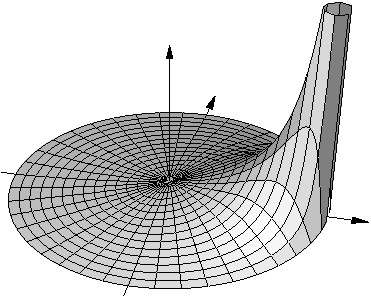
\includegraphics{../figures/poisson-graph}
\end{frame}

\begin{frame}
\begin{proposition}
\begin{enumerate}[(i)]
\item
$P_r(\theta) > 0$ for all $0 \leq r < 1$ and all $\theta$.
\pause
\item
$\int_{-\pi}^{\pi} P_r(\theta) \, d\theta = 1$
for all $0 \leq r < 1$.
\pause
\item
For any given $\delta > 0$,
$\sup \bigl\{P_r(\theta) : \delta \leq \abs{\theta} \leq
\pi \bigr\} \to 0$ as $r \uparrow 1$.
\end{enumerate}
\end{proposition}

\pause

The graph of $P_r$ as a function of $\theta$ on $[-\pi,\pi]$ for
$r=0.5$, $r=0.7$, and $r=0.85$:

\begin{center}
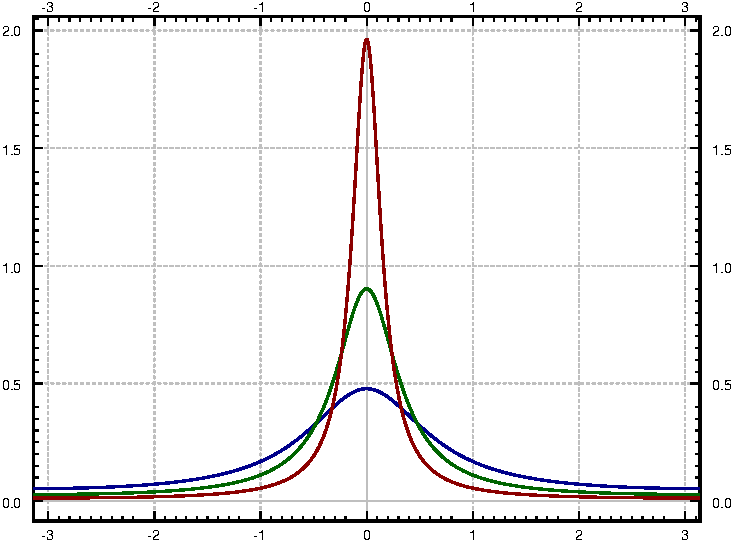
\includegraphics[width=0.45\textwidth]{../figures/poisson-kernel.pdf}
\end{center}

\end{frame}

\begin{frame}
Recall: $
P_r(\theta)
= \frac{1}{2\pi} \frac{1-r^2}{1+r^2-2r \cos \theta}
= \frac{1}{2\pi}
\Re \left( \frac{1+re^{i\theta}}{1-re^{i\theta}}\right) ,
$
\quad
$0 \leq r < 1$.
\pause
\medskip

(i) (positive): \quad $1-r^2 > 0$
\quad
and
\quad
$1+r^2-2r \cos\theta \geq 1+r^2-2r = {(1-r)}^2 > 0$

\medskip
\pause

(ii) (integral is 1):
\[
\int_{-\pi}^{\pi}
P_r(\theta) \, d\theta
\pause
=
\frac{1}{2\pi}
\int_{-\pi}^{\pi}
\Re
\left(
\frac{1+re^{i\theta}}{1-re^{i\theta}}
\right)
\, d\theta
\pause
=
\Re
\frac{1}{2\pi i}
\int_{-\pi}^{\pi}
\frac{1+re^{i\theta}}{1-re^{i\theta}} \frac{1}{re^{i\theta}} \,
ire^{i\theta}
\, d\theta
\hspace*{1in}
\]
\[
\hspace*{1in}
\pause
= 
\Re
\frac{1}{2\pi i}
\int_{\partial \Delta_r(0)}
\frac{(1+z)/(1-z)}{z} \, dz
\pause
\overset{\text{CIF}}{=}
\Re \frac{1+0}{1-0} = 1 .
\]
\pause

(iii) ($\sup \bigl\{P_r(\theta) : \delta \leq \abs{\theta} \leq
\pi \bigr\} \to 0$ as $r \uparrow 1$):


\pause
By symmetry only need to prove for $\delta \leq \theta \leq \pi$.
\pause
\quad
On $(0,\pi)$, $P_r$ is strictly decreasing, so only need to show
that $P_r(\delta) \to 0$.
\pause
\quad
$r \mapsto
\frac{1+re^{i\delta}}{1-re^{i\delta}}$
is continuous at $r=1$ and \pause
\[
\frac{1+e^{i\delta}}{1-e^{i\delta}}
=
\frac{(1+e^{i\delta})(1-e^{-i\delta})}{(1-e^{i\delta})(1-e^{-i\delta})}
\pause
=
\frac{e^{i\delta}-e^{i\delta}}{\sabs{1-e^{i\delta}}^2}
\pause
=
i \frac{2\Im e^{i\delta}}{\sabs{1-e^{i\delta}}^2} . \qed
\]
\end{frame}

\begin{frame}
\begin{theorem}
Let $f \colon \partial \D \to \R$ be continuous.
Then
$Pf \colon \widebar{\D} \to \R$, defined by
\begin{equation*}
%Pf(re^{i\theta})
%=
%\int_{-\pi}^\pi f(e^{it}) P_r(\theta-t) \, dt
%\quad \text{if $r < 1$} \qquad \text{and} \qquad
%Pf(e^{i\theta}) = f(e^{i\theta}),
Pf(re^{i\theta})
=
\begin{cases}
\int_{-\pi}^\pi f(e^{it}) P_{r}(\theta-t) \, dt
&
\text{if $r < 1$,} \\
f(e^{i\theta}) & \text{if $r=1$,}
\end{cases}
\end{equation*}
is harmonic in $\D$ and continuous on $\widebar{\D}$.
\end{theorem}

\pause
\textbf{Proof:}
Let $z = re^{i\theta}$.
\pause
For fixed $t$,
\begin{equation*}
P_r(\theta-t)
\pause
=
\frac{1}{2\pi}
\Re
\left(
\frac{1+re^{i(\theta-t)}}{1-re^{i(\theta-t)}}
\right) 
\pause
=
\frac{1}{2\pi}
\Re
\left(
\frac{1+ze^{-it}}{1-ze^{-it}}
\right)
\end{equation*}
\pause
is harmonic as a function of $z=re^{i\theta}$.
\quad
\pause
\[
Pf(z)
=
Pf(re^{i\theta})
\pause
=
\int_{-\pi}^\pi f(e^{it}) P_r(\theta-t) \, dt
\pause
=
\frac{1}{2\pi}
\int_{-\pi}^\pi f(e^{it}) 
\Re
\left(
\frac{1+z e^{-it}}{1-z e^{-it}}
\right) 
\, dt
\]
\pause
is harmonic for $z = re^{i\theta} \in \D$ (differentiate under the integral).
\end{frame}

\begin{frame}
%Now as both $P_r$ and $f(e^{it})$ is $2 \pi$-periodic we 
%can
%Change variables:
\[
Pf(re^{i\theta})
=
\int_{-\pi}^\pi f(e^{it}) P_r(\theta-t) \, dt
=
\int_{-\pi}^\pi f\bigl(e^{i(\theta-t)}\bigr) P_r(t) \, dt .
\qquad \text{($2\pi$-periodic)}
\]
\pause
Let $\epsilon > 0$ be given.
\pause
\quad
$M = \sup \{ f(z) : z \in \partial \D \}$.
\pause

$f$ uniformly continuous \pause \wthus $\exists$ $\delta > 0$
such that $\abs{f\bigl(e^{i(\theta-t)}\bigr)-f(e^{i\theta})} <
\nicefrac{\epsilon}{2}$ whenever $\sabs{t} < \delta$.

\pause
\medskip

Find 
$\delta' > 0$ such that
\quad $0 < P_r(t) < \frac{\epsilon}{8M\pi}$ \quad
whenever
$1-\delta' < r < 1$ and $\sabs{t} \geq \delta$.
\pause
\[
f(e^{i\theta})=
\int_{-\pi}^\pi f(e^{i\theta}) P_r(t) \, dt 
\qquad \Bigl(\text{as} \ \int_{-\pi}^\pi P_r(t) \, dt = 1\Bigr).
\]
\pause
\[
\sabs{
Pf(r e^{i\theta} ) - f(e^{i\theta})
}
\pause
=
\abs{
\int_{-\pi}^{\pi} \Bigl( f\bigl(e^{i(\theta-t)}\bigr)-f(e^{i\theta}) \Bigr) P_r(t) \, dt
}
\pause
\leq 
\abs{
\int_{-\pi}^{-\delta} \cdots \, dt
}
+
\abs{
\int_{-\delta}^{\delta} \cdots \, dt
}
+
\abs{
\int_{\delta}^\pi \cdots \, dt
} .
\]
\pause
First:
\begin{equation*}
\abs{
\int_{-\pi}^{-\delta} \Bigl( f\bigl(e^{i(\theta-t)}\bigr)-f(e^{i\theta}) \Bigr) P_r(t) \, dt
}
\pause
\leq
\int_{-\pi}^{-\delta} \abs{ f\bigl(e^{i(\theta-t)}\bigr)-f(e^{i\theta}) }
P_r(t) \, dt
\pause
\leq (\pi-\delta) 2M \frac{\epsilon}{8M\pi}
\pause
< \frac{\epsilon}{4} .
\end{equation*}
\pause
The integral from $\delta$ to $\pi$ is exactly the same.
\end{frame}

\begin{frame}
$\displaystyle
\abs{
\int_{-\delta}^{\delta} \Bigl( f\bigl(e^{i(\theta-t)}\bigr)-f(e^{i\theta}) \Bigr) P_r(t) \, dt
}
\pause
\leq
\int_{-\delta}^{\delta} \abs{f\bigl(e^{i(\theta-t)}\bigr)-f(e^{i\theta})}
P_r(t) \, dt
\pause
\leq
\int_{-\delta}^{\delta} \frac{\epsilon}{2} P_r(t) \, dt$

%\hspace*{0.7in}
\smallskip
$\displaystyle
\hspace*{4.0in}
\leq
\int_{-\pi}^{\pi} \frac{\epsilon}{2} P_r(t) \, dt
\pause
=\frac{\epsilon}{2} .
$

\vspace*{-6pt}

\pause
So $1-\delta' < r < 1$ \wthus
$
\sabs{
Pf(r e^{i\theta} ) - f(e^{i\theta})
} \pause
\leq \nicefrac{\epsilon}{4} + \nicefrac{\epsilon}{2} + \nicefrac{\epsilon}{4} =
\epsilon.$

\pause
\thus \quad $Pf(re^{i\theta}) \to f(e^{i\theta})$ uniformly in $\theta$
as $r \uparrow 1$.

\pause
\medskip

Fix $z_0 = e^{i\theta_0} \in \partial \D$ and $\epsilon > 0$.
\quad
\pause
$f = Pf|_{\partial \D}$ is
continuous, so $\exists$ $\delta > 0$ such that

\medskip

$\sabs{\theta-\theta_0} < \delta$ \wthus
$
\sabs{Pf(e^{i\theta})-Pf(e^{i\theta_0})} < \nicefrac{\epsilon}{2}$

\medskip
\pause

For possibly smaller
$\delta$

\medskip

$1 - \delta < r \leq 1$ \wthus 
$\sabs{Pf(re^{i \theta})-Pf(e^{i\theta})} < \nicefrac{\epsilon}{2}$
\quad for all $\theta$.

\medskip
\pause
So if $z=re^{i\theta}$ satisfies $1 - \delta < r \leq 1$ and
$\sabs{\theta-\theta_0} < \delta$,

\medskip
\pause

$
\sabs{Pf(re^{i\theta})-Pf(e^{i\theta_0})}
\leq
\babs{Pf(re^{i\theta})-Pf(e^{i\theta})}
+
\babs{Pf(e^{i\theta})-Pf(e^{i\theta_0})}
 < \epsilon$.

\vspace{-1.15in}
\hspace*{4in}
\scalebox{0.85}{
\subimport*{../figures/}{proofofdirichlet.pdf_t}
}


\medskip
\pause

\thus \quad
$Pf$ is continuous at $z_0$.
\qed

\medskip
\pause

Remark: We used polar coordinates (homeomorphism near $z_0$).
\end{frame}

\begin{frame}
Translation and scaling gives (proof an exercise):

\begin{corollary} \label{cor:dirichsol}
Let $f \colon \partial \Delta_R(p) \to \R$ be continuous.
Then
$Pf \colon \overline{\Delta_R(p)} \to \R$, defined by
\begin{equation*}
Pf(p + re^{i\theta})
=
\begin{cases}
\int_{-\pi}^\pi f(p+Re^{it}) P_{r/R}(\theta-t) \, dt
&
\text{if $r < R$,} \\
f(p+Re^{i\theta}) & \text{if $r=R$,}
\end{cases}
\end{equation*}
is harmonic in $\Delta_R(p)$ and continuous on $\overline{\Delta_R(p)}$.
\end{corollary}
\pause

Represents harmonic functions like Cauchy integral formula:

\medskip

If $f$ is harmonic on a neighborhood of $\overline{\Delta_R(p)}$
\wthus
$P[f|_{\partial \Delta_R(p)}] = f|_{\overline{\Delta_R(p)}}$.

\medskip
\pause

However, the Poisson kernel above is specific to the disk.

\medskip
\pause

A quick consequence: 
If $f$ is harmonic on a neighborhood of $\overline{\Delta_R(p)}$,
then
\[
f(p) = \frac{1}{2\pi} \int_{-\pi}^{\pi}f(p + R e^{it}) \, dt .
\]
\end{frame}

\begin{frame}
Poisson kernel works for holomorphic functions
(holomorphic functions are harmonic).

\medskip
\pause

For general functions
$Cf$ and $Pf$ are different in the disc:

\medskip

Consider $f(z) = z+\bar{z} = 2\Re(z)$ on the unit circle.

\medskip

$Pf(z) = z+\bar{z}$ \qquad $Cf(z) = z$


\end{frame}

\begin{frame}
\textbf{Exercise:}
Given a bounded continuous $f \colon \R \to \R$, prove that 
$Pf \colon \overline{\bH} \to \R$,
\begin{equation*}
Pf(x+iy)
=
\begin{cases}
\frac{1}{\pi}
\int_{-\infty}^{\infty} f(t) \frac{y}{{(x-t)}^2+y^2} \, dt
&
\text{if $y > 0$,} \\
f(x) & \text{if $y=0$,}
\end{cases}
\end{equation*}
is harmonic in $\bH$ and continuous on $\overline{\bH}$.

\medskip
\pause

\textbf{Exercise:}
Derive the \emph{Schwarz integral formula}, which recovers
a holomorphic function out of the real parts of the boundary values
and the value of the imaginary part at one point.
If $f \colon \overline{\D} \to \C$ is continuous and holomorphic on
$\D$, then for all $z \in \D$,
\begin{equation*}
f(z) =
\frac{1}{2\pi i}
\int_{\partial \D}
\frac{\zeta+z}{\zeta-z} \frac{\Re f(\zeta)}{\zeta} \, d\zeta
+ i \Im f(0) .
\end{equation*}


\end{frame}

\end{document}
